%%%%%%%%%%%%%%%%%%%%%%%%%%%%%%%%%%%%%%%%%%%%%%%%%%%%%%%%%%%%%%%%%%%%%%
% LaTeX Template: Two Column Colour Article
%
% Source: http://www.howtotex.com/
% Feel free to distribute this template, but please keep the
% referal to howtotex.com.
% Date: Feb 2011
% 
%%%%%%%%%%%%%%%%%%%%%%%%%%%%%%%%%%%%%%%%%%%%%%%%%%%%%%%%%%%%%%%%%%%%%%
% How to use overleaf.com: 
%
% You edit the source code here on the left, and the preview on the
% right shows you the result within a few seconds.
%
% You can upload figures, bibliographies, custom classes and
% styles using the files menu.
%
% If you're new to LaTeX, the wikibook is a great place to start:
% http://en.wikibooks.org/wiki/LaTeX
%
%%%%%%%%%%%%%%%%%%%%%%%%%%%%%%%%%%%%%%%%%%%%%%%%%%%%%%%%%%%%%%%%%%%%%%
% adaptions made by wolfgang stoettner mail@stoettner.net
%%%%%%%%%%%%%%%%%%%%%%%%%%%%%%%%%%%%%%%%%%%%%%%%%%%%%%%%%%%%%%%%%%%%%%

%%% Preamble
\documentclass[	DIV=calc,%
							paper=a4,%
							fontsize=11pt,%
							twocolumn]{scrartcl} % KOMA-article class
\usepackage[french]{babel}	% English language/hyphenation
\usepackage[protrusion=true,expansion=true]{microtype}	% Better typography
\usepackage{amsmath,amsfonts,amsthm} % Math packages
\usepackage{pythontex} % Math packages
\usepackage[pdftex]{graphicx} % Enable pdflatex
\usepackage{wrapfig} % enable figure wrapping
\usepackage[svgnames]{xcolor} % Enabling colors by their 'svgnames'
\usepackage[hang, small,labelfont=bf,up,textfont=it,up]{caption} % Custom captions under/above floats
\usepackage{epstopdf} % Converts .eps to .pdf
\usepackage{subfig}	% Subfigures
\usepackage{booktabs} % Nicer tables
\usepackage{fix-cm}	% Custom fontsizes
\usepackage{booktabs} % prof. looking tables (www.en.wikibooks.org/wiki/LaTeX/Tables#Professional_tables)
\usepackage{float}
\usepackage{tgtermes}
\usepackage[T1]{fontenc}
\usepackage[utf8]{inputenc}
\usepackage{pdfpages}
\usepackage[smartEllipses]{markdown}
\usepackage{tikz}
\usetikzlibrary{math}
\usetikzlibrary{shapes.misc}
\usetikzlibrary{arrows.meta,decorations.markings} % arrow and decorations
%%% Custom sectioning (sectsty package)
\usepackage{sectsty} % Custom sectioning (see below)
\allsectionsfont{%		% Change font of al section commands
	\usefont{OT1}{phv}{b}{n}%	% bch-b-n: CharterBT-Bold font
	}

\sectionfont{%		% Change font of \section command
	\usefont{OT1}{phv}{b}{n}%	% bch-b-n: CharterBT-Bold font
	}
%%% Headers and footers
\usepackage{fancyhdr} % Needed to define custom headers/footers
	\pagestyle{fancy} % Enabling the custom headers/footers
\usepackage{lastpage}	

% Header (empty)
\lhead{}
\chead{}
\rhead{\today}
% Footer (you may change this to your own needs)
\lfoot{\footnotesize \texttt{formulaire capteur} \textbullet \vspace{5pt} Antonin Kenzi}
\cfoot{}
\rfoot{\footnotesize page \thepage\ of \pageref{LastPage}}	% "Page 1 of 2"
\renewcommand{\headrulewidth}{0.0pt}
\renewcommand{\footrulewidth}{0.4pt}
\newcommand{\hformbar}[1]{\bigskip\hrule\vspace{5pt}} % creates a horizontal bar to separate formulae better; space adaptions can be made centrally here


%%% Creating an initial of the very first character of the content
\usepackage{lettrine}
\newcommand{\initial}[1]{%
     \lettrine[lines=3,lhang=0.3,nindent=0em]{
     				\color{DarkGoldenrod}
     				{\textsf{#1}}}{}}

%%% Title, author and date metadata
\usepackage{titling} % For custom titles

\newcommand{\HorRule}{\color{DarkGoldenrod}%	% Creating a horizontal rule
									  	\rule{\linewidth}{1pt}%
										}
\pretitle{\vspace{-30pt} \begin{flushleft} \HorRule 
				\fontsize{15}{15} \usefont{OT1}{phv}{b}{n} \color{DarkRed} \selectfont 
				}
\title{Formulaire Reg Num} % Title of your article goes here
\posttitle{\par\end{flushleft}}
\preauthor{\vspace{-20pt} \begin{flushleft}\large \usefont{OT1}{phv}{b}{sl} \color{DarkRed}}
\author{Kenzi Antonin}	% Author name goes here
\postauthor{\vspace{-20pt} \footnotesize \usefont{OT1}{phv}{m}{sl} \color{Black}  \par\end{flushleft}\HorRule}
\date{\vspace{-30pt} \today} % No date
\newcounter{mycounter}
%%% wws: create a non-indented formula name
\newcommand{\formdesc}[1]{\noindent\textbf{#1} \addtocounter{mycounter}{1} \hfill \themycounter}

%%% Begin document -----------------------------------------------------------------
\begin{document}
\maketitle
\thispagestyle{fancy} 	% Enabling the custom headers/footers for the first page 
% The first character should be within \initial{}

\formdesc{Concept}

3 objectif à la régulation : 
\begin{enumerate}
    \item Stable
    \item Rapide 
    \item Bien amorti
\end{enumerate}

Deux genres de régulation :
\begin{enumerate}
    \item Correspondance : signal y(t) suit la consigne w(t)
    \item maintien : signal y(t) devrait ne pas ou peu être influencé par les perturbations v(t)
\end{enumerate}
\hformbar

\formdesc{Différence analogique/numérique}

3 objectifs à la régulation : 
\\
\begin{tabular}{c|c}
    Analogique & Numérique \\ \hline
    Signaux temp u(t), y(t) & signaux temp u[k], y[k]\\ \hline
    signaux fréq U(s), Y(s) & signaux fréq U(z), Y(z)\\ \hline
    transformée en s&  transformée en z\\ \hline
    équations différentielles&  équation aux différences\\ \hline
    fonction de transfert :&fonction de transfert :\\ 
    $G(s) = Y(s) / U(s)$& $G(z) = Y(z) / U(z)$\\ \hline
    gain statique : G(s=0) &gain statique : G(z=1)\\ \hline
    pôles, zéros, & pôles, zéros, \\ \hline
    diagr. de Bode&diagr. de Bode\\ \hline
    stabilité : $Re(s_k)$ < 0&stabilité : $|z_k| < 1$\\ 
    (demi-plan gauche)&(int. du cercle unit.)\\ \hline
\end{tabular}
\hformbar

\formdesc{Régulateur Numérique}

Cours 1 page 5
\hformbar


\formdesc{Échantillonnage}

Cours 1 page 6-8
\hformbar

\formdesc{Inventaire des retards}

Cours 1 page 15-19
Cours 3 page 1-6
\hformbar


\formdesc{Rappel Nyquist et méthode pôles dominants}

Cours 2 page 1-3
\hformbar

\formdesc{schéma et FTZ intégrateur}

Cours 2 page 4-8
\hformbar

\formdesc{Inventaire des retards}

Cours 1 page 15-19
\hformbar

\formdesc{Inventaire des retards}

Cours 1 page 15-19
\hformbar

\formdesc{Lieu des poles(Root locus)}

\footnotesize Outil important permettant la synthèse de systèmes réglés : 
\begin{enumerate}
 \item choix de Kp 
\end{enumerate}

pôles complexes conjugués :

{\hfill $s_{1,2} = -\delta \pm j\omega $\hfill}

Réponse indicielle :

{\hfill $g(t) = e^{-\delta \cdot t} \cdot sin(\omega t) $\hfill}

Rappel (formulaire régulation automatique) : 

{\hfill $T_{reg} = \cfrac{3}{\delta} = \cfrac{-3}{\mathbb{R}(s_f)}$\hfill}\vspace{3mm}

Règles de tracer du lieu des pôles (L.d.P) :
\begin{enumerate}
    \item L.d.P a n branches = degré du dénominateur 
    \item L.d.P a M branches = degré du numérateur
    \item L.d.P symétrique par l'axe $\mathbb{R}$
    \item Points de départ à $K_p = 0$
    \item Points de fin à $K_p = \infty$
    \item $d = n-m$ branches restante partent en asymptote infinie, où d correspond au degré relatif de la B.O\\ les asymptotes forment des étoiles régulières
    \item Tout point de l'axe réel situé à gauche d'un nombre impair de pôles et de zéros réels fait partie du lieu
\end{enumerate}

\tikzset{cross/.style={cross out, draw=black, minimum size=2*(#1-\pgflinewidth), inner sep=0pt, outer sep=0pt},
cross/.default={4pt}}

\tikzset{ % this style creates an arrow like the one you draw in the middle of a path
   ->-/.style={decoration={markings,mark=at position 0.5 with {\arrow{Straight Barb}}},
               postaction={decorate}}
}
%default radius will be 1pt. 
\begin{tikzpicture}[]
    \tikzmath{
    coordinate \x;
    \x1=(-2,0);
    \x2=(0,0);
    \x3=(-2.5,0);
    \x4 = (-3,0);
    \x5 = (-1,0);
    }
    
    \draw[help lines,dashed] (-5.5,-1.5) grid (0.5,1.5);
    \draw[->] (-6,0) -- (1,0) node [anchor=west] {$R$};
    \draw[->] (0,-1.5) -- (0,1.5) node [anchor=south] {$Img$};
    \draw[->-,red,thick] (\x1) -- (\x5);
    \draw[->-,red,thick] (\x5) arc (0:180:1);
    \draw[->-,red,thick] (\x4) -- (\x3);
    
    \draw[->-,blue,thick] (\x2) -- (\x5);
    \draw[->-,blue,thick] (\x5) arc (0:-180:1);
    \draw[->-,blue,thick] (\x4) -- (-6,0);
    \draw (\x1) node[cross] {};
    \draw (\x2) node[cross] {};
    \draw (\x3) circle (4pt);
    
\end{tikzpicture}


\hformbar



%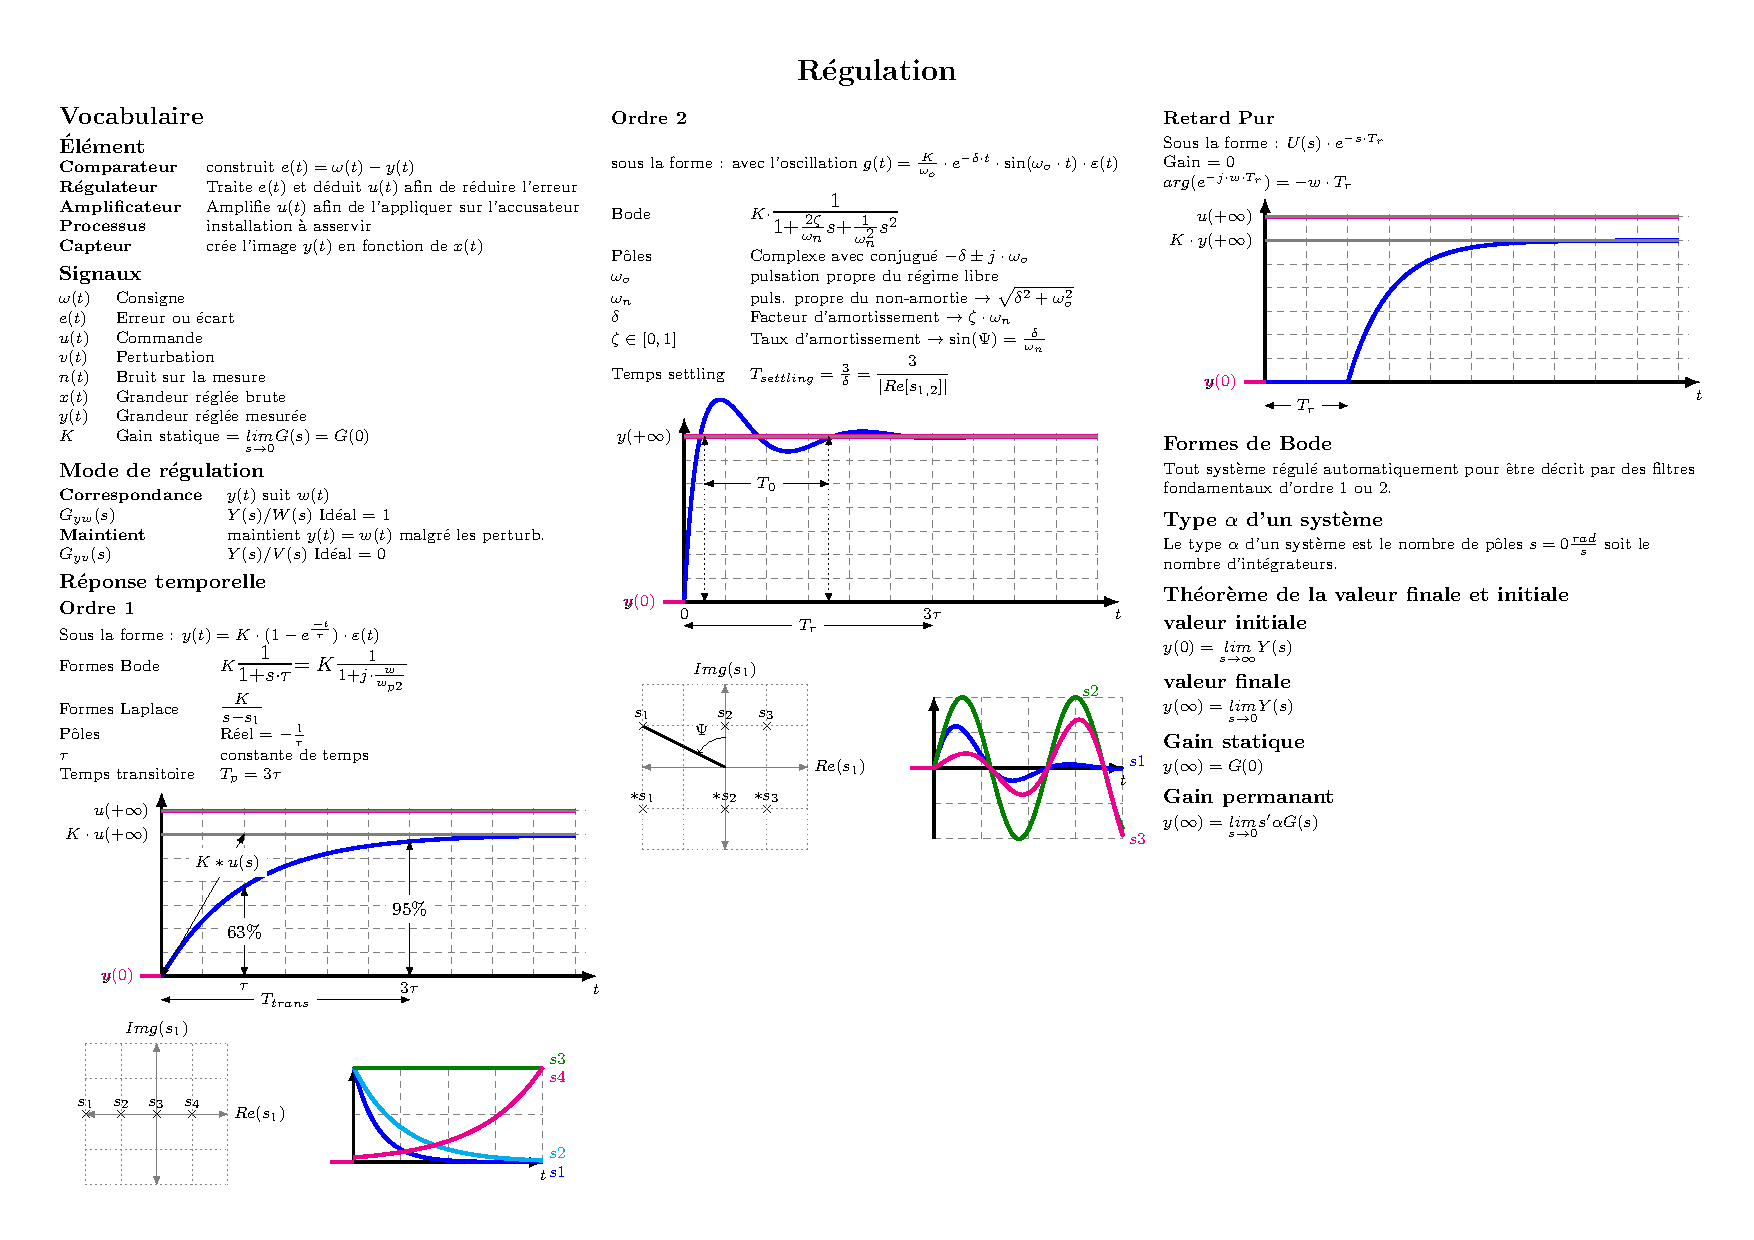
\includepdf[pages=-]{img/cheat.pdf}

\end{document}